% !TEX root = comparison-review.tex
\subsection{Study I: Wind Direction and Airport Efficiency}
\subsubsection{Setup}
The data contains all flights \cite{rita} in and out of Seattle/Tacoma International Airport (SEA) between July 2008 and June 2011. As a measure of airport efficiency we are using time between successive wheel-events (time at wheel take-off or touch-down), which we found to be independent of airline carrier and operating hours, as long as we restricted the data to `regular' operating hours between 7 am and midnight and `regular' weather conditions -- i.e. we eliminated records associated with the top 5\% wind speed measurements \cite{noaa-weather}, leaving us with just under half a million flights.

In this scenario, all of the lineups are testing the null hypothesis 

\vspace{-0.1in}
\begin{quote}
$H_0: $ {\em wind direction has no effect on efficiency }
\end{quote}
\vspace{-0.1in}

\noindent against the alternative $H_a:$ {\em wind direction does have an effect.}

Statistical tests of mean efficiency by wind direction are not particularly helpful in this situation: the difference in mean efficiency between the  wind direction at which the airport operates the most efficiently and its least efficient direction shows a statistically significant difference with a $p$-value $\le 10^{-15}$. %2.2e-16$.  
However, out of the 34 other wind directions,  another 31 show significant differences in efficiency as well. This is much more a property of the large data size rather than practically usable differences. Mere significances also do not allow us an assessment of the underlying pattern.

In deciding on the design for displaying efficiency by wind direction we were using the fact that wind direction is circular, and  displayed the data as (conditional) wind rose charts - i.e. for each of 36 wind directions we show the percentage of flights falling into one-minute intervals between successive flights, from  zero minutes to eight minutes or more.

\begin{figure}[htbp] %  figure placement: here, top, bottom, or page
%   \centering
 \hspace{-.1in}
   \begin{tabular}{ccl}
   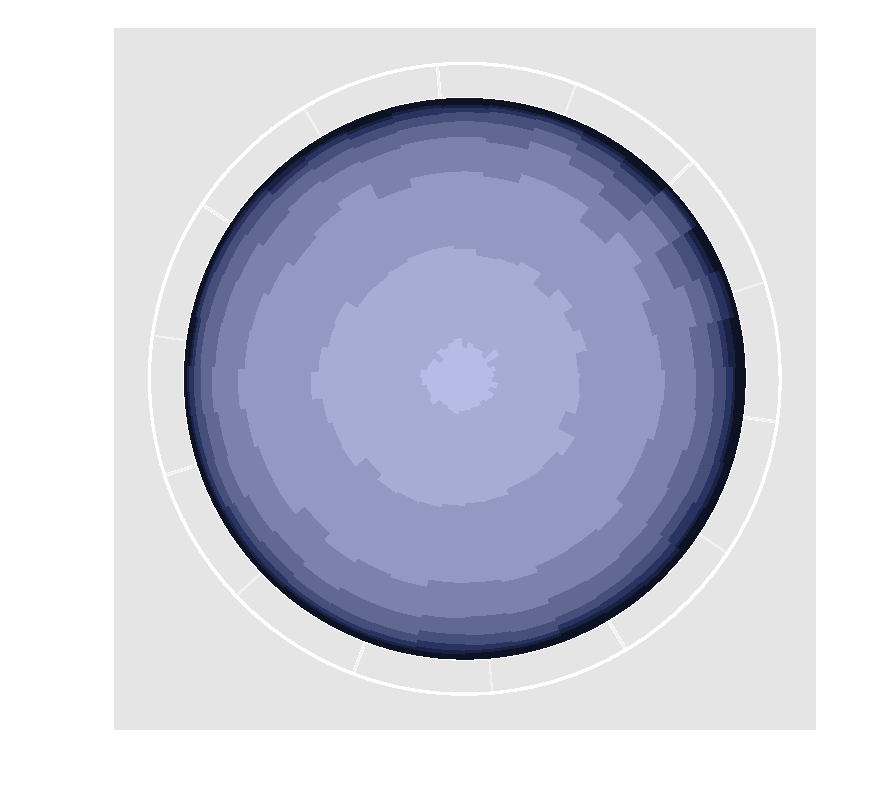
\includegraphics[width=0.43\linewidth]{Polar_NoLine.pdf} &  \hspace{-.3in}
   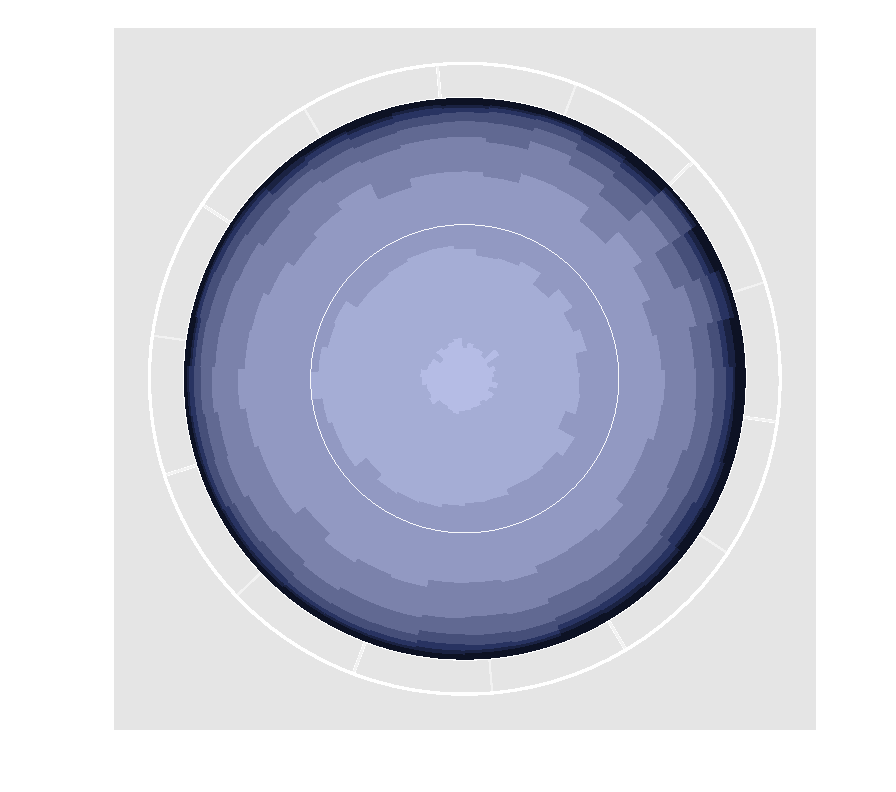
\includegraphics[width=0.43\linewidth]{Polar_Line.pdf}  &  \hspace{-.2in} \multirow{2}{*}[.55in]{  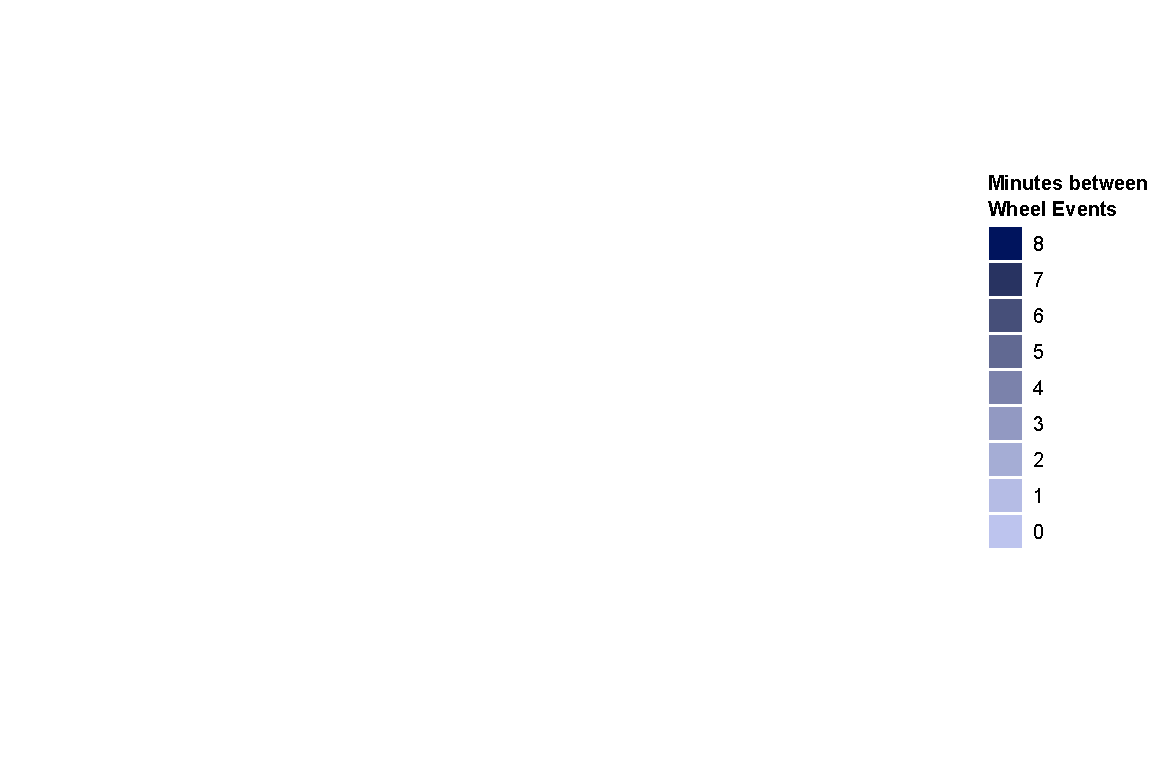
\includegraphics[width=0.2\linewidth]{legend.pdf}} \\
   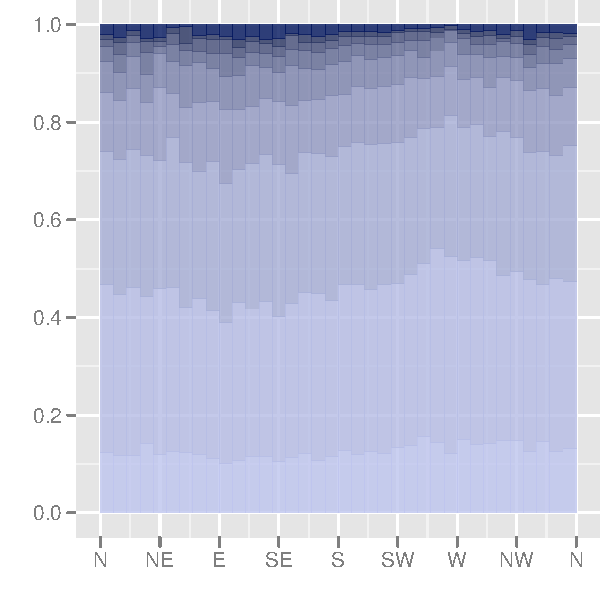
\includegraphics[width=0.375\linewidth]{euclid_noline.pdf} & \hspace{-.3in}
   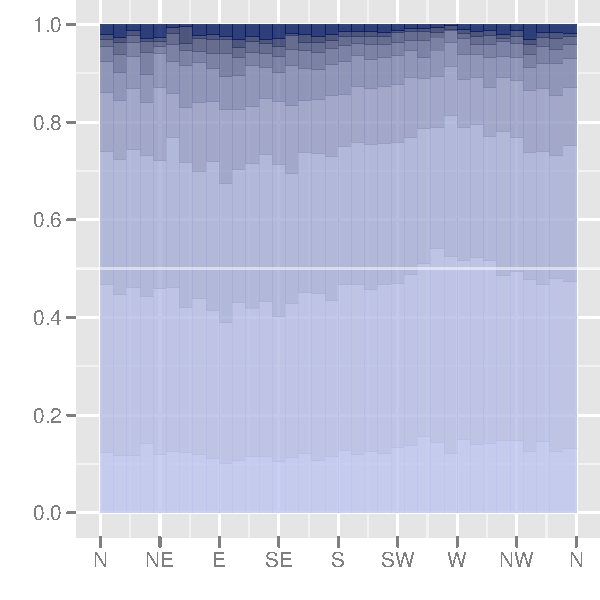
\includegraphics[width=0.375\linewidth]{euclid_line.pdf}
   \end{tabular}
\vspace{-.2in}
   \caption{All four competing designs: polar versus cartesian charts in top and bottom row, with (right) and without (left) reference lines at 50\%. }
   \label{layouts}
\end{figure}

In spite of the contextual circular property of wind direction, the pattern in efficiency did not seem to stand out well during the exploration process, which led us to using a corresponding  cartesian design. Both designs were additionally equipped with a reference line at 50\%. 
Figure \ref{layouts} shows an overview of all four chart types in the study. During the exploration of the data, it became clear that Seattle airport functions most efficiently with winds coming from the east to southeast, while winds from the west seemed to be most troublesome, resulting in a wave-like pattern in the cartesian charts and a shift in center for the polar charts. Since runways can be used in both directions, changing the runway usage according to dominant wind direction for that day or time of the year might be a feasible solution in gaining efficiency. 

An additional factor we were interested in this particular situation was to assess, how much of the data we actually needed to use in a design to have observers pick out the pattern. Clearly, a design is more efficient, if a smaller sample size is sufficient for showing the presence of a relationship. In order to investigate this, we took different size samples of the data and created lineup plots of all four designs for these subsets. The effect of sample size on the displays mostly stems from the additional variability introduced when using small samples, which might hide the pattern, if it is not displayed prominently. 

Another perturbation to the data are `shifts' in wind direction, i.e. we make use of the circular nature of the wind direction and adjust the $x$ axis by using different offsets.

\begin{figure}[htbp] %  figure placement: here, top, bottom, or page
   \centering
   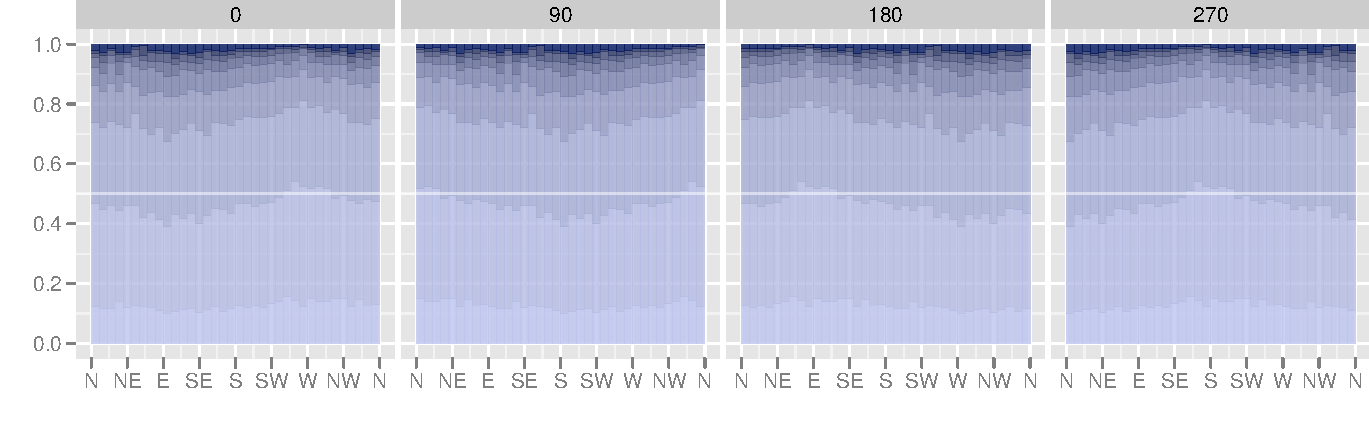
\includegraphics[width=\linewidth]{euclid-offset} 
   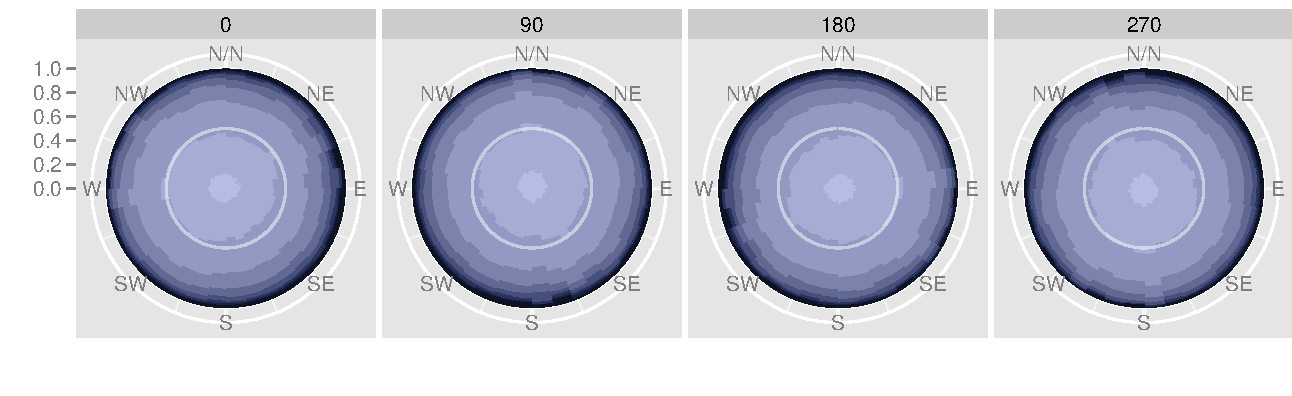
\includegraphics[width=\linewidth]{polar-offset} 
   \caption{ \label{fig:offset} (Top) Cartesian charts of the same sample, with shifts in wind direction by 90, 180, and 270 degrees. The shift by 90 and 270 leads to a `valley' versus a `mountain' pattern, whereas a shift by 180 degrees inverts the wave pattern from `down-up' to `up-down'. %\hfill\newline
      (Bottom) Shifts in wind direction in the polar chart lead to rotations of the display by 90 degrees.}
\end{figure}

 This results in a shift of the wave in cartesian charts and a rotation in the polar charts as can be seen in Figure \ref{fig:offset}. Our initial thinking was that this would have no effect on the polar charts, but might have a deteriorating effect on the cartesian charts, in the case that the peak or the valley of the wave was at either end of the $x$ axis, i.e. an offset of 90 or 270 degrees. 
While these simple perturbations and different sample sizes allow us to get insight into different aspects of the designs, they also allow us to get multiple responses from each observer to assess individual ability without the need to go outside the framework of the original data, i.e. we leave the joint relationship between $x$ and $y$ essentially unchanged. For all of these combinations we produced two replicates, resulting in a total of 192 different lineups ($ 4 \text{ designs} \times 6 \text{ sample sizes} \times 4 \text{ offsets} \times 2 \text{ reps})$.
Table \ref{tbl:treatment} gives an overview of the number of times lineups in each combination of design and sample size were shown, and in how many of them the data plot was correctly identified. 

\begin{table}[hbtp]
\centering
%\resizebox{\linewidth}{!} {
	%\rowcolors{1}{white}{lightgray}
	\begin{tabular}{ll@{   }r@{   }r@{   }r@{   }r@{   }r@{   }r}
	& & \multicolumn{6}{c}{sample size}  \\
        \multicolumn{2}{l}{type of chart} & 2 & 4 & 6 & 8 & 10 & 24 \\ [1pt] \hline 
	cartesian & with & 12/{\bf 24}& 18/{\bf 27} & 42/{\bf 44} & 33/{\bf 41} & 39/{\bf 43} & 46/{\bf 47}\\
	       &      &(0.50)& (0.67) & (0.95) & (0.80) & (0.91) & (0.98)\\[1pt]
	& without & 13/{\bf 41} &24/{\bf 32}& 39/{\bf 44} & 47/{\bf 51} & 40/{\bf 45} & 34/{\bf 37}\\
	&         & (0.32) &(0.75)& (0.89) & (0.92) & (0.89) & (0.92)\\[3pt] %\hline
	polar & with & 13/{\bf 49}& 9/{\bf 43} & 9/{\bf 39} & 7/{\bf 35} & 8/{\bf 40} & 13/{\bf 38} \\
	      &      & (0.27)& (0.21) & (0.23) & (0.20) & (0.20) & (0.34) \\[1pt]
	& without & 6/{\bf 51}&   4/{\bf 34} &  5/{\bf 34} &  6/{\bf 39} & 11/{\bf 43} &  12/{\bf 37} \\
        &         & (0.12) & (0.12) &  (0.15) &  (0.15) & (0.26) &  (0.32)\\ 
	\end{tabular}
%	}
\caption{\label{tbl:treatment} Breakdown of lineups: number correct/\textbf{number shown} (proportion correct). Each participant was shown eight lineups, and the same lineup was shown to multiple people (denominator in the table) reasonably well-spread among the treatment levels. }
\end{table}

%Besides correctness of responses, two additional response variables were recorded:  time taken for answer and a (subjective) confidence level, ranging from 1 (lowest) to 5 (highest), assessing how convinced participants are of the correctness of their answer. 

%\begin{table}[ht]
%\begin{center}
%%\resizebox{\linewidth}{!} {
%\rowcolors{2}{white}{lightgray}
%\begin{tabular}{rrrrr}
%  \hline
% & Estimate & Std..Error & t.value & pval \\ 
%  \hline
%(Intercept) & 2.92 & 0.16 & 18.17 & 0.00 \\ 
%  polar & -0.30 & 0.16 & -1.86 & 0.06 \\ 
%  reflineTRUE & -0.16 & 0.09 & -1.74 & 0.08 \\ 
%  sample\_size & 0.01 & 0.01 & 1.01 & 0.31 \\ 
%  offset90 & 0.14 & 0.13 & 1.07 & 0.28 \\ 
%  offset180 & 0.03 & 0.13 & 0.26 & 0.80 \\ 
%  offset270 & 0.01 & 0.12 & 0.07 & 0.94 \\ 
%  polar:reflineTRUE & 0.31 & 0.13 & 2.46 & 0.01 \\ 
%  polar:sample\_size & -0.01 & 0.01 & -0.70 & 0.49 \\ 
%  polar:offset90 & -0.14 & 0.18 & -0.78 & 0.44 \\ 
%  polar:offset180 & -0.01 & 0.18 & -0.04 & 0.97 \\ 
%  polar:offset270 & -0.00 & 0.18 & -0.01 & 0.99 \\ 
%   \hline
%\end{tabular}
%%}
%\end{center}
%\caption{\label{tbl:confidence} Model output for confidence level. }
%\end{table}

%%
%%The goal of this experiment is to understand the efficiency of displaying information using euclidian and polar coordinates. Efficiency is the deviation from independence, which can be simulated by taking permutations of the original dataset. Data concerning wind patterns and time between flights at SEA airport is used for these charts. The lineup chart is composed of 20 graphics with all of the exact same characteristics except for the data. One of the 20 graphics will be using original airport data while the other 19 will be permutations of that data. Efficiency of the chart types can be inferred by how accurately individuals pick out the plot with the original data. There are other variables which are introduced to further our understanding of the way we perceive euclidian and polar coordinates. All combinations of each level of the variables are involved in the experiment for both polar and euclidian coordinates. The graphics in each chart will all have exactly the same level of the variables with the only difference being the data. 
%%
%%The other variables which are monitored are existence of reference line, placement of x-axis, and sample size. It is possible that one of the chart types benefits more from additional components such as reference lines. The polar and euclidian null charts will be shown either with or without a white reference line. The line is placed at slightly over 50 percent of the y axis. Additionally, the x-axis has four placements. The original dataset contains a characteristic wave pattern, which for euclidian coordinates, may be a large factor contributing to the perceived effectiveness of the graphic. Characteristic patterns such as the wave pattern may be perceived in a different way when viewed in polar coordinates. When the x-axis is is shifted the look of the pattern changes. The wave pattern is broken up for euclidian coordinates but for polar coordinates is only shifted around the axis. Finally, the amount of information necessary for detection as well as correctness is a measure for efficiency of the charts so the sample size which was taken from the original dataset is of interest. The original data set contained XXX,XXX observations from which 2, 4, 6, 8, 10, and 24 percent of the observations were sampled. Small sample sizes are easier to obtain because of time and money constraints. It would be nice to know if there is one type of chart which can show data trends using less information. 
%%
%%
%% All combinations of these variables were repeated for plots with a reference line and without a reference line, as shown in figure \ref{layouts}.This figure shows examples of graphics showing the actual data, which in the experiment would be randomly positioned among 19 null plots. In total there are XXX unique charts which represent all different combinations of sample size, coordinate type, x-axis placement, and whether or not there is a reference line. The charts are all assigned a difficulty level, which is based on sample size, on a scale from zero to four. There are two plots assigned a difficulty level of zero. These two charts, one polar and one Euclidian, were made from computer generated data and intended to be at the level where an individual, if he or she is not purely guessing, should be able to find the correct plot. 
%%
%%
%%Amazon's Mechanical Turk is an online service in which individuals can request and perform simple tasks and surveys for money. Using Turk we were able to gather data on how people responded to the charts. Each person is shown a series of ten charts and asked to choose the graphic on each chart which they think is "different". They then identify, from a list of choices, why they chose this particular chart as well as how confident they are on a scale of one to five. Personal information such as age group, gender, and education is also collected on a voluntary basis. The amount of time it took the individual to answer is also recorded. This study allows us to make informed judgments about how the plot type effects efficiency in terms of accuracy and time spent reading the plots. Xcite stephen few?X
%%Effect is deviation from independence. Cannot be properly measured statistically except in highly aggregated situations, where the effect might be washed out.
%%
%%Most generally this experiment can be paralleled to the pie chart versus barchart discussion. The Euclidian coordinate plot is made up of bars *whose?* areas are colored proportionally according to the data. The polar coordinate plot is made up of pie slices which are also colored proportionally according to the data. Viewers of these charts will visually decode the areas of the bars and pie slices and make a judgement based on their decoding. How accurate this judgment is is left to be discussed. According to  \cite[page=40]{kosslyn:2006}, area is usually perceived as a function of what the actual area is. This function is the area raised to an exponent of approximately 0.8 and then multiplied by a constant. However, when bars are parallel, the relative height of these bars is perceived very accurately. From this information, one could infer that the Euclidian coordinate plot may gain efficiency based on the height of the colored bars. 
%%Pie versus Barchart discussion is pretty old: cite some of the literature:
%%
%%From Stephen Few, perceptual edge:
%%	When a graph is made, quantitative and categorical information is encoded by a display method. Then the information is visually decoded. This visual perception is a vital link. No matter how clever the choice of the information, and no matter how technologically impressive the encoding, a visualization fails if the decoding fails. Some display methods lead to efficient, accurate decoding, and others lead to inefficient, inaccurate decoding. It is only through scientific study of visual perception that informed judgments can be made about display methods. (William S. Cleveland, The Elements of Graphing Data, Hobart Press, 1994, p. 1)
%%	
%%	The systematic distortion of area is captured by �Steven�s Power Law,� which states that the psychological impression is a function of the actual physical magnitude raised to an exponent (and multiplied by a scaling constant). To be precise, the perceived area is usually equal to the actual area raised to an exponent of about 0.8, times a scaling constant...In contrast, relative line length [such as the lengths of bars] is perceived almost perfectly, provided that the lines are oriented the same way \cite[page=40]{kosslyn:2006}

%%	
%%	
%%	We make angle judgments when we read a pie chart, but we don�t judge angles very well. These judgments are biased; we underestimate acute angles (angles less than 90�) and overestimate obtuse angles (angles greater than 90�). Also, angles with horizontal bisectors (when the line dividing the angle in two is horizontal) appear larger than angles with vertical bisectors. (Naomi Robbins, Creating More Effective Graphs, Wiley, 2005, p. 49)
%%	
%%	 Edward Tufte once said that �the only worse design than a pie chart is several of them, for then the viewer is asked to compare quantities located in spatial disarray both within and between pies� (Edward Tufte, The Visual Display of Quantitative Information, Graphics Press, 1983, p. 178.)
%%
%% We do not claim to settle the question - which is multi-facetted and will not have a clear 'winning' design but instead very much depends on the purpose of the chart and task at hand.

\subsubsection{Results for Study I}

Figures \ref{fig:time} and \ref{fig:conf} give an overview of the relationship between the three response variables: accuracy, speed, and confidence level.

Figure \ref{fig:time} shows histogram of the time participants needed to make a decision on each lineup. Correctness of answers is shown by color.  Because of the skewness of the distributions, times were log-transformed. Polar charts take on average more time to answer, and are answered with much lower accuracy. 
The average amount of time spent on a cartesian lineup is $e^{3.53} = 34.1$ seconds compared to $e^{4.07}=58.5$ seconds for a polar lineup.
This is in stark contrast to accuracy: 76.92\% of the cartesian lineups shown resulted in the a correct identification of the real data while only 20.31\% of the polar charts were correct.


\begin{figure}[hbtp] %  figure placement: here, top, bottom, or page
   \centering
   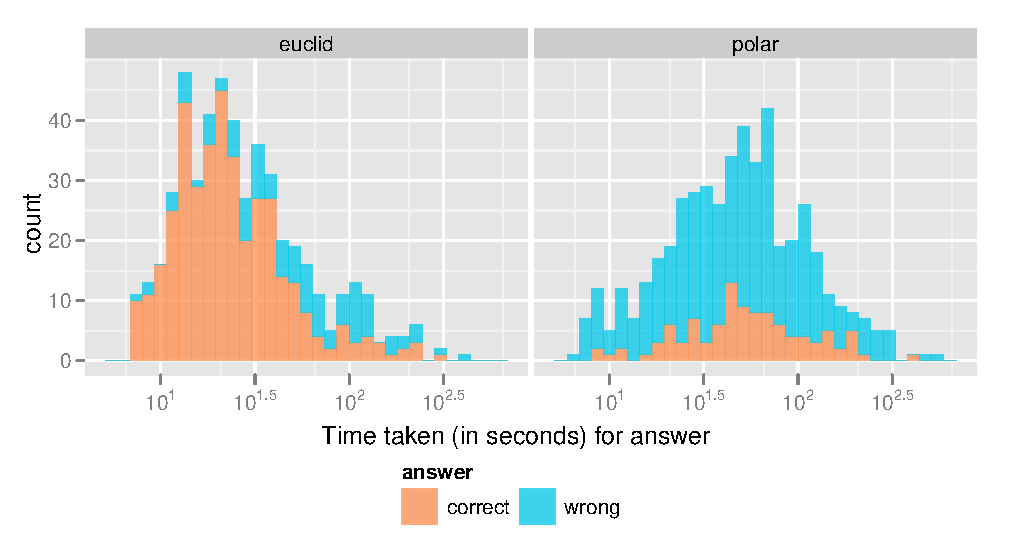
\includegraphics[width=.95\linewidth]{time-answer} 
   \caption{Histograms of time taken for answering lineups. On average the cartesian design is answered faster and with higher precision.}
   \label{fig:time}
\end{figure}

Figure \ref{fig:conf} shows two barcharts of confidence levels by task, again coloring is used for correctness of answers. Cartesian displays lead to a very bimodal distribution of confidence: participants are either very sure or not sure at all of their answer. Confidence levels in polar charts are distributed much more uniformly. Confidence levels seem to be independent from precision, though.
\begin{figure}[hbtp] %  figure placement: here, top, bottom, or page
   \centering
   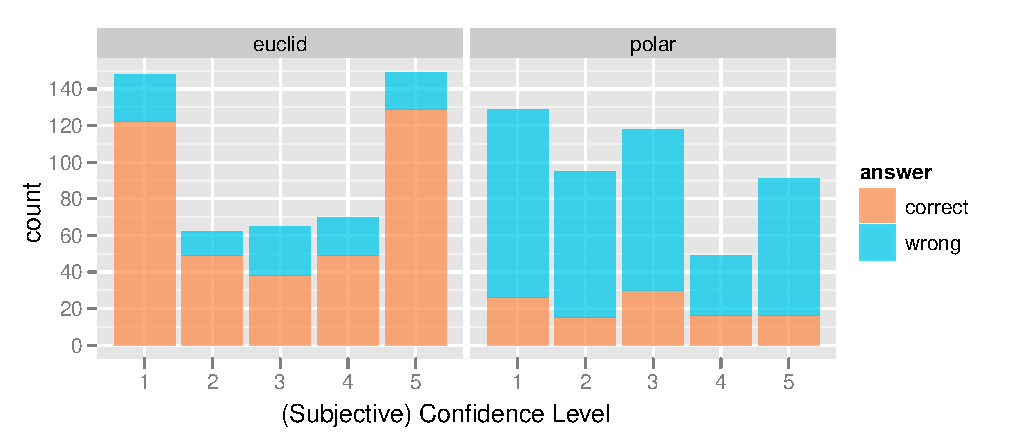
\includegraphics[width=.95\linewidth]{conf-answer} 
\vspace{-0.2in}
   \caption{Barcharts of self-reported confidence in answering correctly for each lineup. A strongly bimodal distribution is apparent, while confidence levels for polar charts are more uniform. Confidence levels are not indicative of accuracy: none of the differences between confidence levels show a significant difference in accuracy.}
   \label{fig:conf}
\end{figure}

%The two methodologically sound
%  studies of pie charts vs. bar charts were done by Simkin and Hastie in a
%  detailed JASA article and Spence and Lewandowsky in a psychology journal.
%
%These are also the only authors
%  to develop and test a coherent cognitive theory of why this is the case
%  (and, I will add in an ad hominem, they are the only pie researchers
%  professionally trained to address this problem in all its complexity).
%  All the other references are either anecdotal, based on faulty
%  methodology, or inappropriate generalizations of irrelevant experimental
%  findings. I feel especially strongly about this point because there is no
%  place in an academic paper for perpetuating a myth that over-generalizes
%  Cleveland's finding for angles (which have no relation to the slices of a
%  pie). Finally, the only similarity between the polar charts in this study
%  and pie charts is that they are both in polar coordinates. There is no
%  point in mentioning pie charts at all.

%The perceptual tasks involved in decoding the designs fit into the general framework of the piechart versus barchart discussion. However, we are not dealing with assessing angles, which is known to be perceptually harder than assessments of heights or widths in bars, see e.g. \cite{cleveland:1984, robbins:2004, Kosslyn:2006, few:2009}. Instead, t
The perceptual involved in decoding the designs consist of comparisons along a common axis (in the barcharts) and a common origin (in the polar charts). The difference in designs is therefore based on how well we are able to judge deviations from a horizontal line compared to deviations from a circle. Based on this, the charts with added reference lines provide us with exactly the frame we compare with and should, therefore, be the `better' designs - either in speed or accuracy.

Figure \ref{fig:treatment} shows a comparison of power for the four competing designs. 95\% confidence intervals are  Bonferroni adjusted for multiple testing. The bottom two confidence intervals in each panel show a 95\% confidence interval of a direct comparison of the cartesian design versus the polar design with and without a reference line. With the exception of the 2\% sample none of those confidence intervals include the zero, indicating a significantly higher power for the cartesian design than for the polar design.

\begin{figure}[htbp] %  figure placement: here, top, bottom, or page
%   \centering

\begin{tabular}{cl}
\phantom{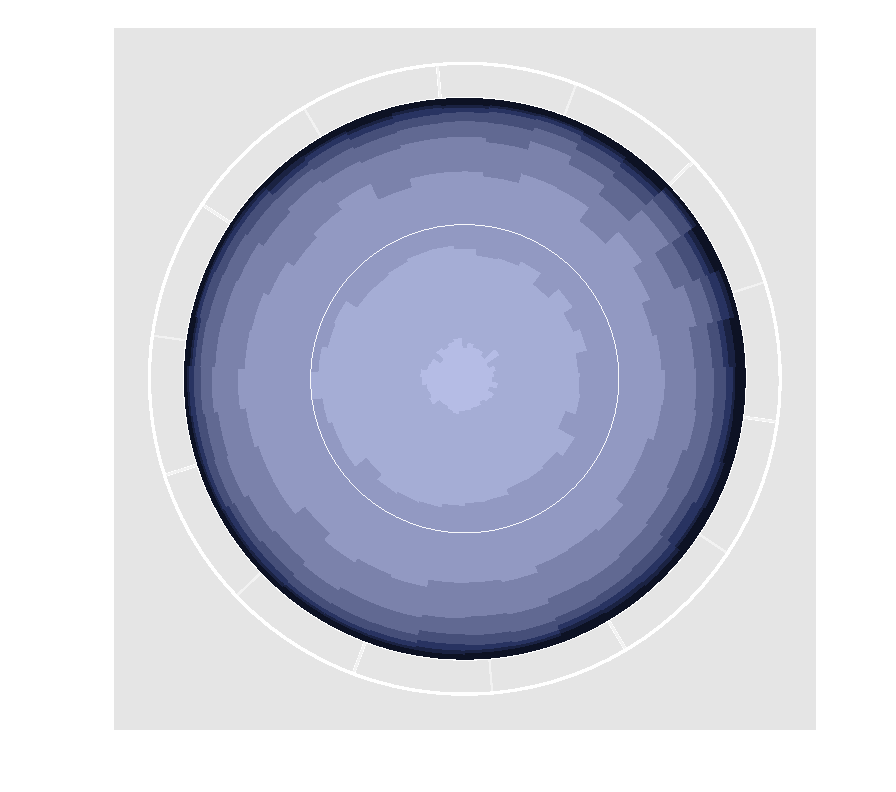
\includegraphics[width=0.03\linewidth]{Polar_Line.pdf}} & \vspace{-0.035in} \multirow{10}{*}{\hspace{-0.4in}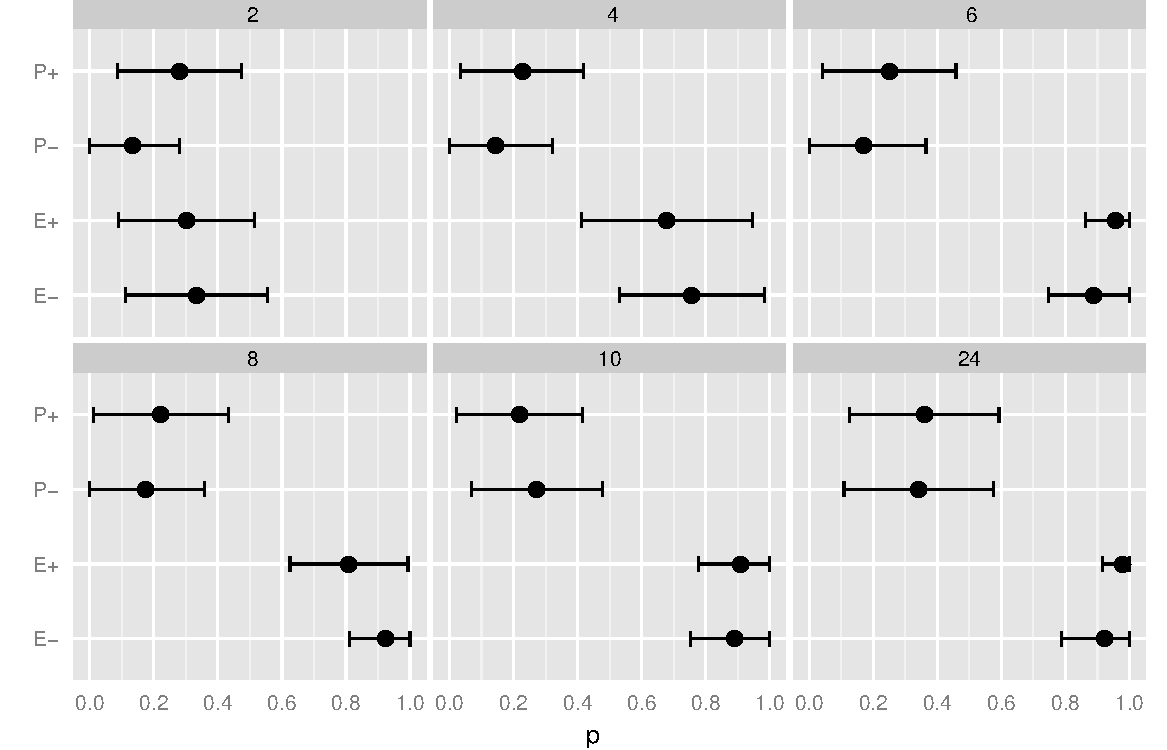
\includegraphics[width=0.9\linewidth]{turk4-designs.pdf}} \\
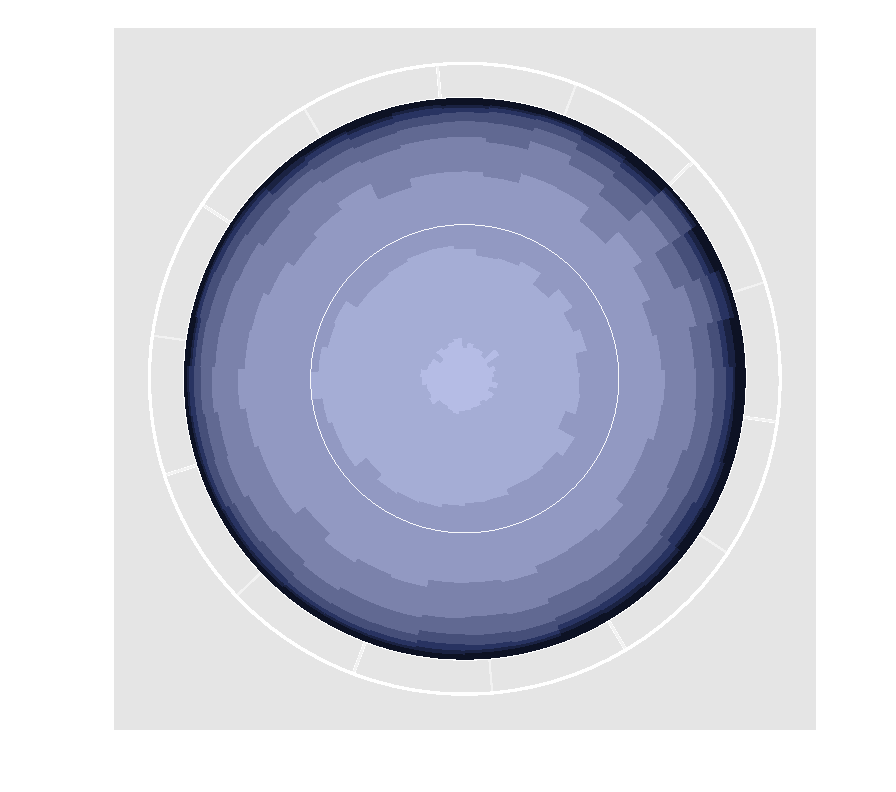
\includegraphics[width=0.045\linewidth]{Polar_Line.pdf} \\
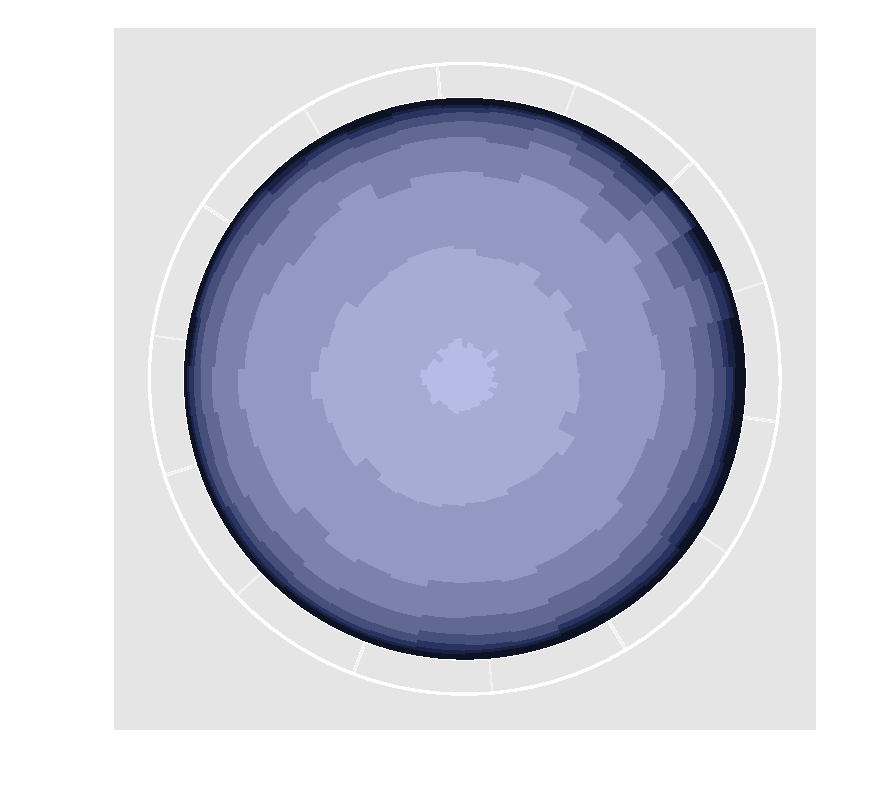
\includegraphics[width=0.045\linewidth]{Polar_NoLine.pdf} \\
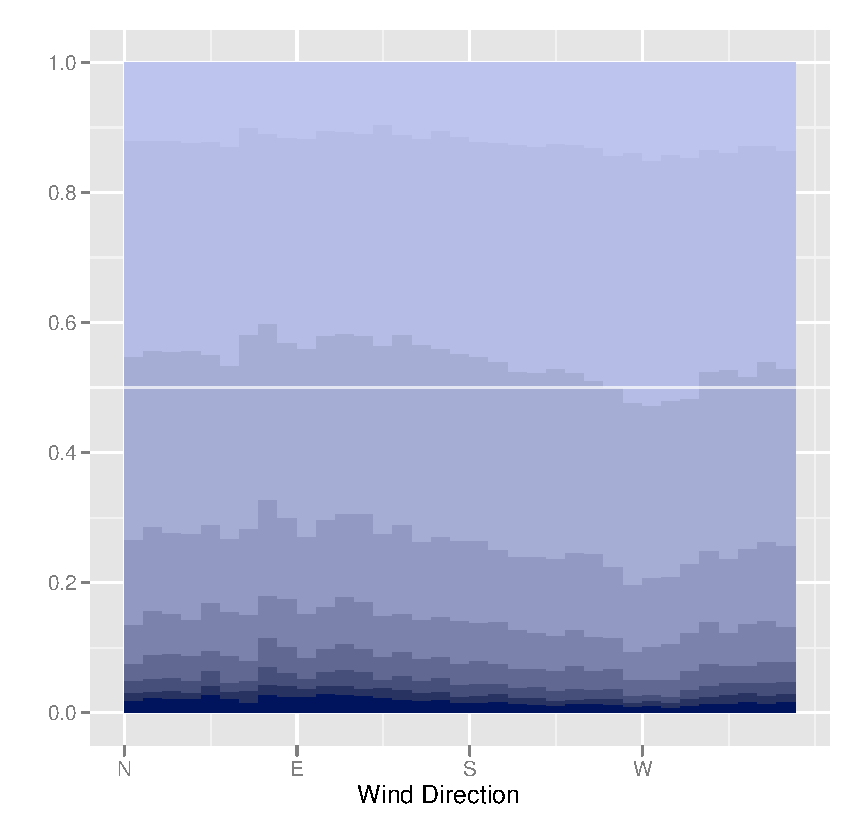
\includegraphics[width=0.043\linewidth]{Euclidian_Line.pdf} \\
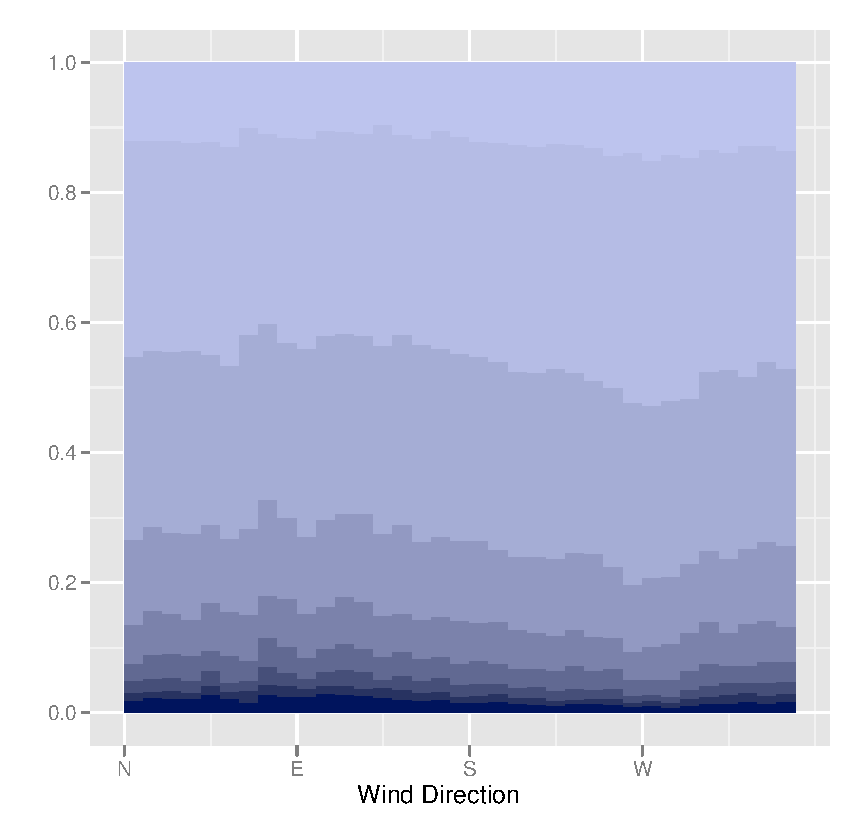
\includegraphics[width=0.043\linewidth]{Euclidian_NoLine.pdf}\\[10pt]
%\phantom{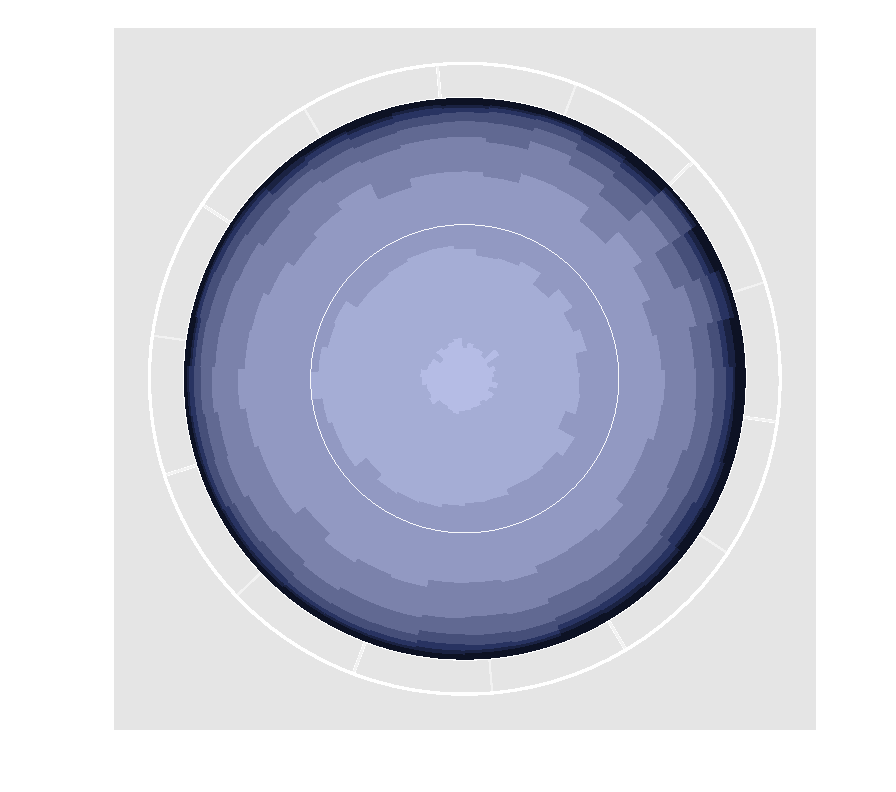
\includegraphics[width=0.13\linewidth]{Polar_Line.pdf}}\\
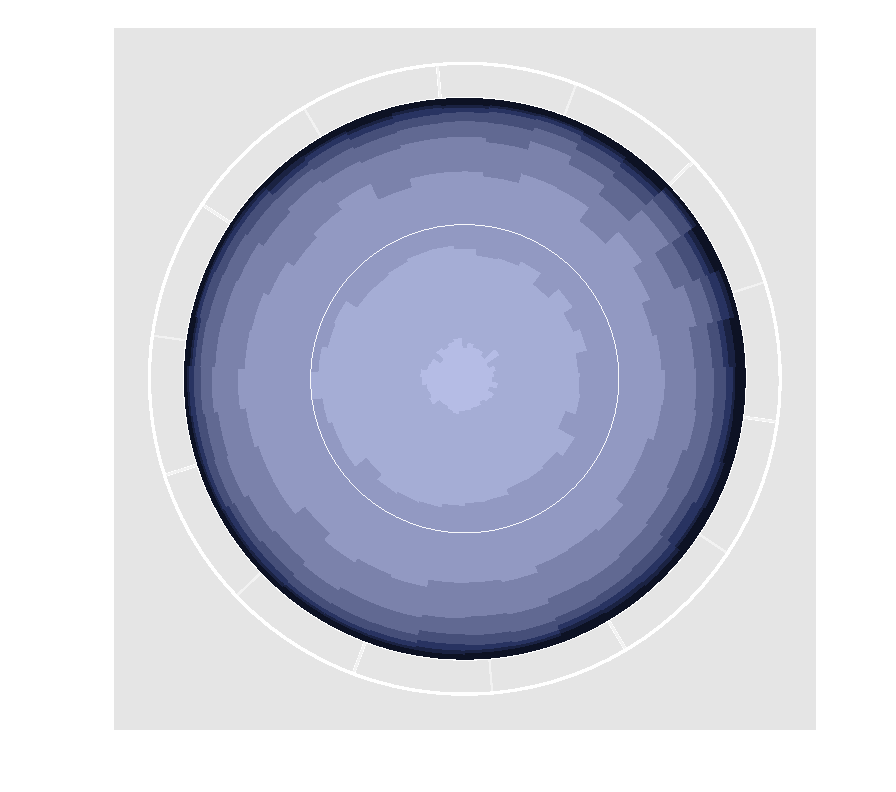
\includegraphics[width=0.045\linewidth]{Polar_Line.pdf} \\
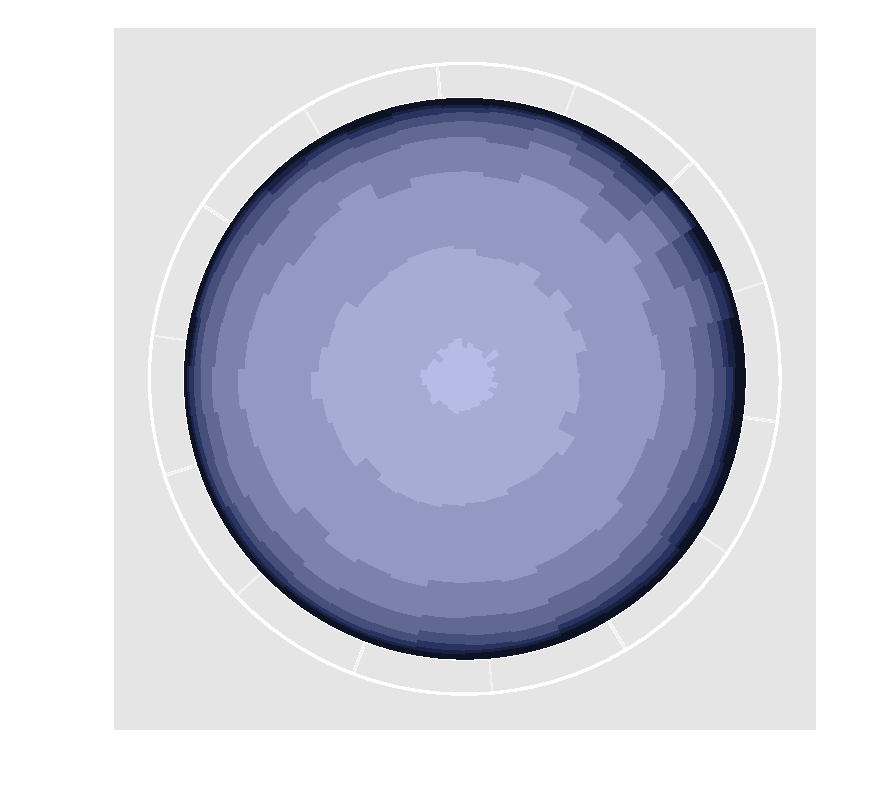
\includegraphics[width=0.045\linewidth]{Polar_NoLine.pdf} \\
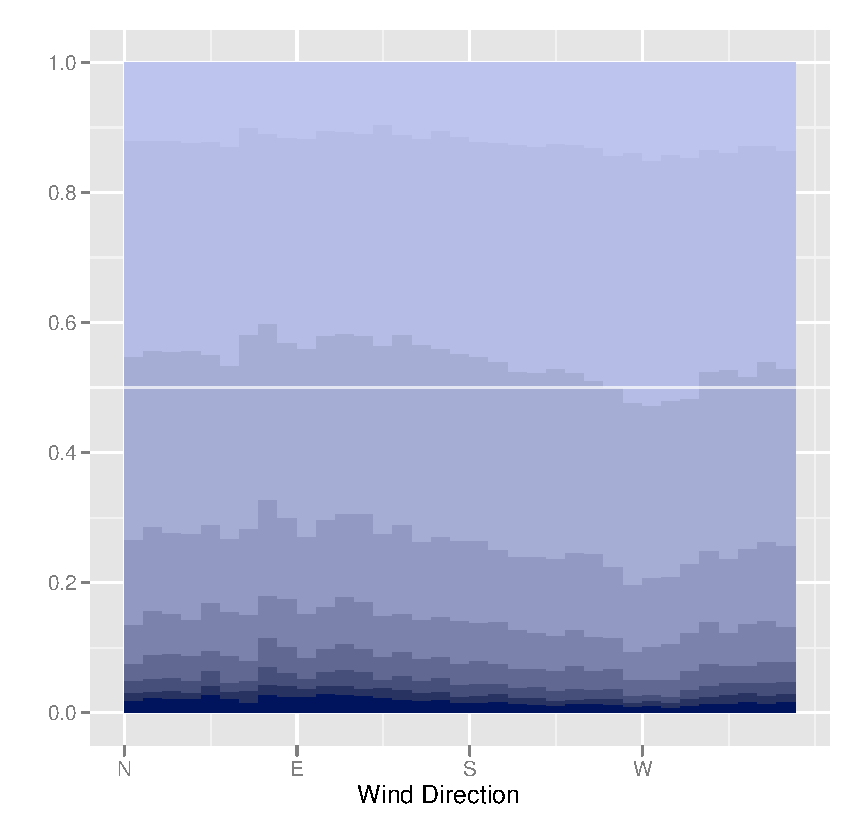
\includegraphics[width=0.043\linewidth]{Euclidian_Line.pdf} \\
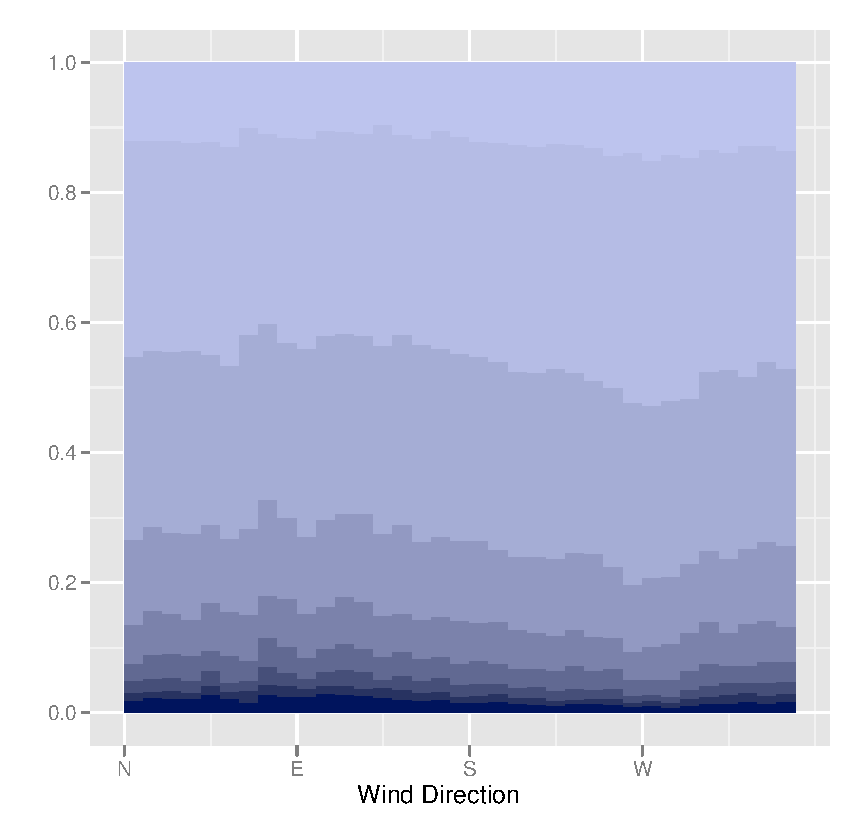
\includegraphics[width=0.043\linewidth]{Euclidian_NoLine.pdf}\\
\phantom{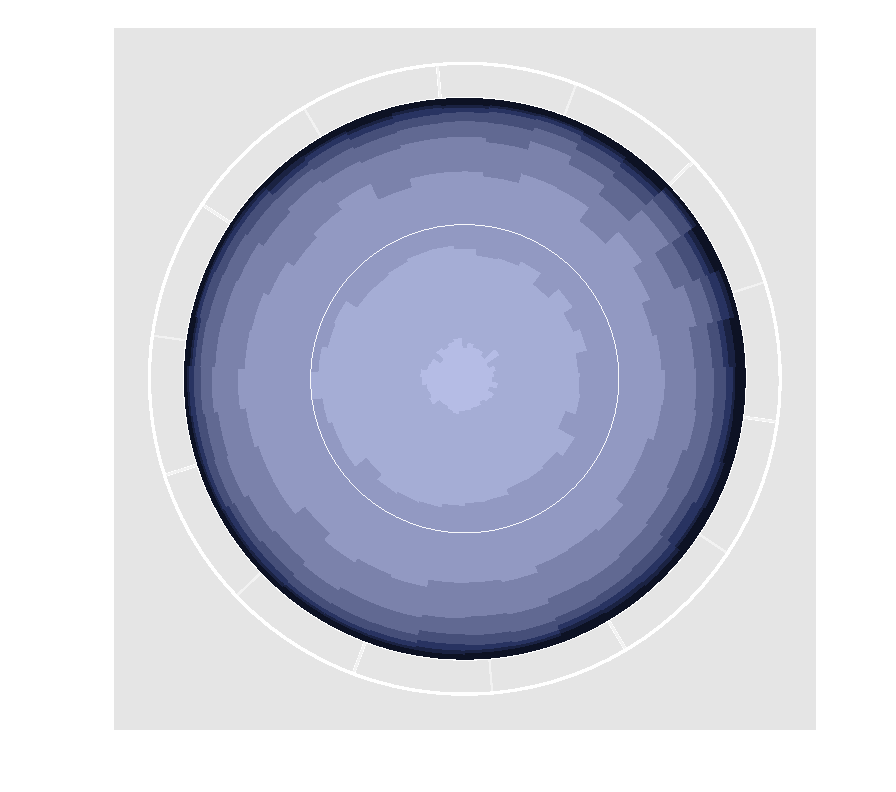
\includegraphics[width=0.13\linewidth]{Polar_Line.pdf}}\\
  \end{tabular} 
  \vspace{-0.35in}
   \caption{Power results for four competing designs: polar versus  cartesian, each with and without a reference line; panels are facetted by sample size (as percentage of original data). Dots show estimated power, surrounded by intervals of standard errors.
 The letters at the front of each panel allow comparisons across all designs  \citep{piepho:2004}: all designs with different letters have significantly different  power  (at $\alpha=0.05$). This is adjusted for all pairwise comparisons using a Benjamini-Hochberg adjustment \citep{bh:1995, hothorn:2010}.
%
%   Error bars indicate single Bonferroni adjusted 95\% confidence intervals. The two confidence intervals at the bottom of each panel shows a pairwise power comparison of cartesian versus polar design according to eqn (\ref{eq:comp}). Differences from zero (vertical grey line) are of interest.
   }
   \label{fig:treatment}
\end{figure}



%Most generally this experiment can be paralleled to the pie chart versus barchart discussion \cite{***}. 
%The cartesian coordinate plot is made up of bars where areas are colored proportionally according to percentages. The polar coordinate plot is made up of pie slices which are also colored proportionally according to the data. 
%Viewers of these charts will visually decode the areas of the bars and pie slices and make a judgement based on their decoding. According to  \citet[page=40]{kosslyn:2006}, area is usually perceived as a function of what the actual area is. This function is the area raised to an exponent of approximately 0.8 and then multiplied by a constant. However, when bars are parallel, the relative height of these bars is perceived very accurately. From this information, one could infer that the cartesian coordinate plot may gain efficiency based on the height of the colored bars. 


However, all of these considerations are based on the - rather strong - assumption that all individuals have the same ability to detect the data plot from a lineup. In order to allow for individual differences in visual ability, 
 we use a generalized linear mixed effects modeling  approach \cite{pinheiro:2000} for each of the three response values, using the {\tt R} package {\tt lme4} \cite{bates:2011}. 
For power predictions (cf. table \ref{tbl:correct}) a logistic regression was fitted for the competing designs, including covariates {\it sample size} (2, 4,6, 8, 10, and 24 percent of the data) and {\it shift} in wind direction (offset of 0, 90, 180, and 270 degrees), both as main effects and in two-way interaction effects with design to assess their effect on the power of designs. To adjust for individuals' ability, a random intercept was included in the model.

\begin{table}[ht]
\begin{center}
\resizebox{\linewidth}{!} {
%\rowcolors{2}{white}{lightgray}
\begin{tabular}{rrrrrrl}
  \hline
& & Estimate & Error & $z$-value & $p$-value &\\ 
  \hline
\bf design & cartesian & -0.08 & 0.39 & -0.21 & 0.84 &\\ 
&polar & -1.98 & 0.32 & -6.13 & 0.00 & ***\\ [3pt]
\multicolumn{2}{l}{\bf main effects} &&&&&\\
& reference line  & -0.14 & 0.26 & -0.53 & 0.59 & \\ [1pt]
&  sample size & 0.27 & 0.04 & 6.31 & 0.00 & ***\\[1pt]
 &offset:  90 degrees& -0.43 & 0.37 & -1.18 & 0.24 &\\ 
  & 180 degrees& -0.89 & 0.35 & -2.51 & 0.01 & **\\ 
  & 270 degrees& 0.21 & 0.38 & 0.55 & 0.58 &\\ [3pt]
\multicolumn{2}{l}{\bf interactions} &&&&&\\
&  polar:line & 0.51 & 0.35 & 1.44 & 0.15 &\\ [1pt]
&    polar:sample size & -0.23 & 0.05 & -5.02 & 0.00 & ***\\[1pt]
&    polar:offset 90 & 0.64 & 0.49 & 1.30 & 0.20 \\ 
&  polar:offset 180 & 0.91 & 0.47 & 1.92 & 0.05 & .\\ 
&    polar:offset 270 & -0.73 & 0.54 & -1.35 & 0.18 &\\
   \hline
\\[-5pt]
   \multicolumn{5}{l}{Signif. codes:  0 `***' 0.001 `**' 0.01 `*' 0.05 `.' 0.1}
\end{tabular}
}
\end{center}
\vspace{-0.2in}
\caption{\label{tbl:correct} Output of a generalized linear mixed effects model for power of lineups (i.e. probability of identifying the data plot) for comparing designs. Included are two-way interactions with sample size and shifts in wind direction (offset). Cartesian designs without a reference line at offset 0 are used as baseline.
 Results are based on  976 lineup evaluations by 115 participants. }
\end{table}

%Note that we excluded demographic information about individuals (i.e., age, gender and education level), as none of these covariates exhibited any significant relationship with accuracy while adding to model complexity. 


Overall, the results show huge differences in the power of designs between polar charts and cartesian: cartesian designs are significantly more powerful than polar charts, particularly so with small sample sizes. 
 The reference line has surprisingly little influence, but it helps more for  polar charts than for cartesian charts,
An increase in sample size has a positive impact on power. Polar charts need a much bigger sample size to see an increase in power -- only at about 24\% of the original data do we see about the same power as for cartesian charts of a sample size of 2\%.
The  changes in offset are significant -- interestingly, borderline behavior (90 and 270 degrees) does not show a difference between polar and cartesian charts, whereas an inversion of the wave pattern (first up, then down), does show a difference. The power of cartesian lineups suffers significantly  from this inversion whereas power of polar charts is unaffected. This is an unexpected finding, but is consistent throughout different lineups in the data. Figure \ref{fig:power} summarizes the results from the model: power predictions ($y$ axis) are shown by sample size ($x$ axis). The thick lines show average power by design for different shifts in wind direction. The thin lines represent power for individuals. What can be seen is the different impact of the offset by design: while  an offset of 270 degrees (the `mountain' pattern) has the highest power in cartesian charts, it comes out worst in polar charts.

\begin{figure}[htbp] %  figure placement: here, top, bottom, or page
   \centering
   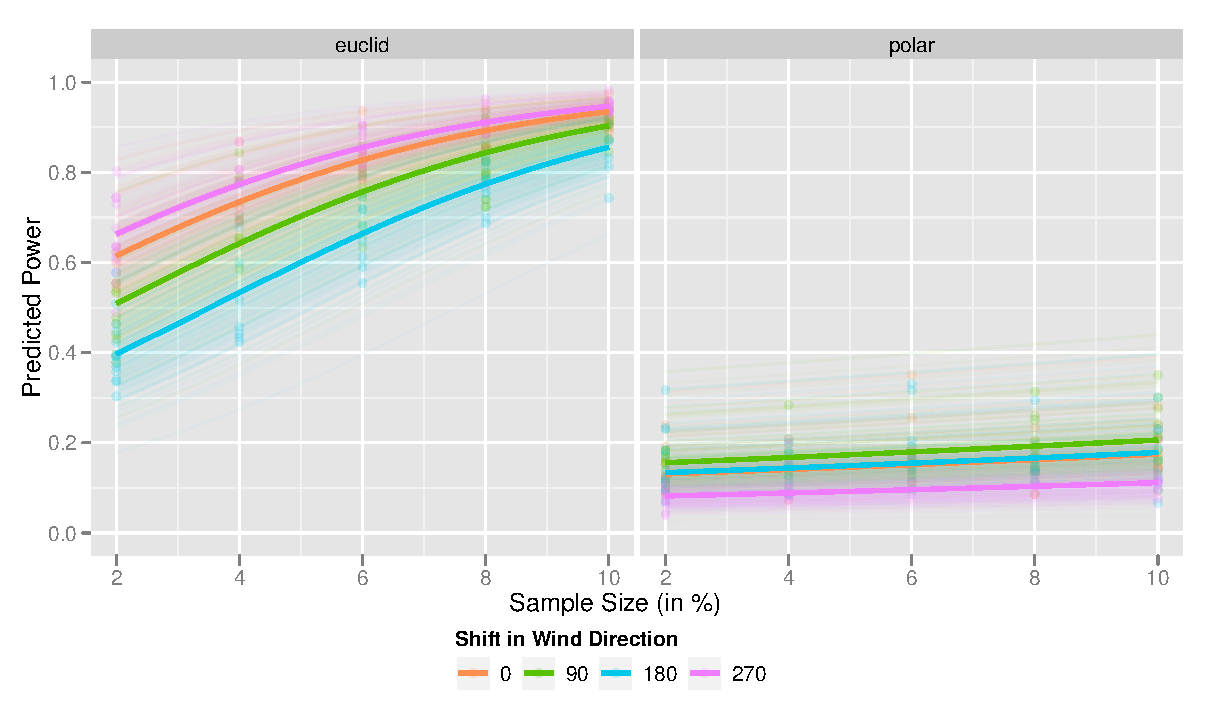
\includegraphics[width=0.95\linewidth]{predict-power} 
\vspace{-0.2in}
   \caption{Predicted Power of designs.  The thin lines and the points on $y$ axis show  variability due to individuals' abilities. The saturated lines show average predicted power for each of the designs.}
   \label{fig:power}
\end{figure}

\begin{figure*}[hbtp] %  figure placement: here, top, bottom, or page
   \centering
   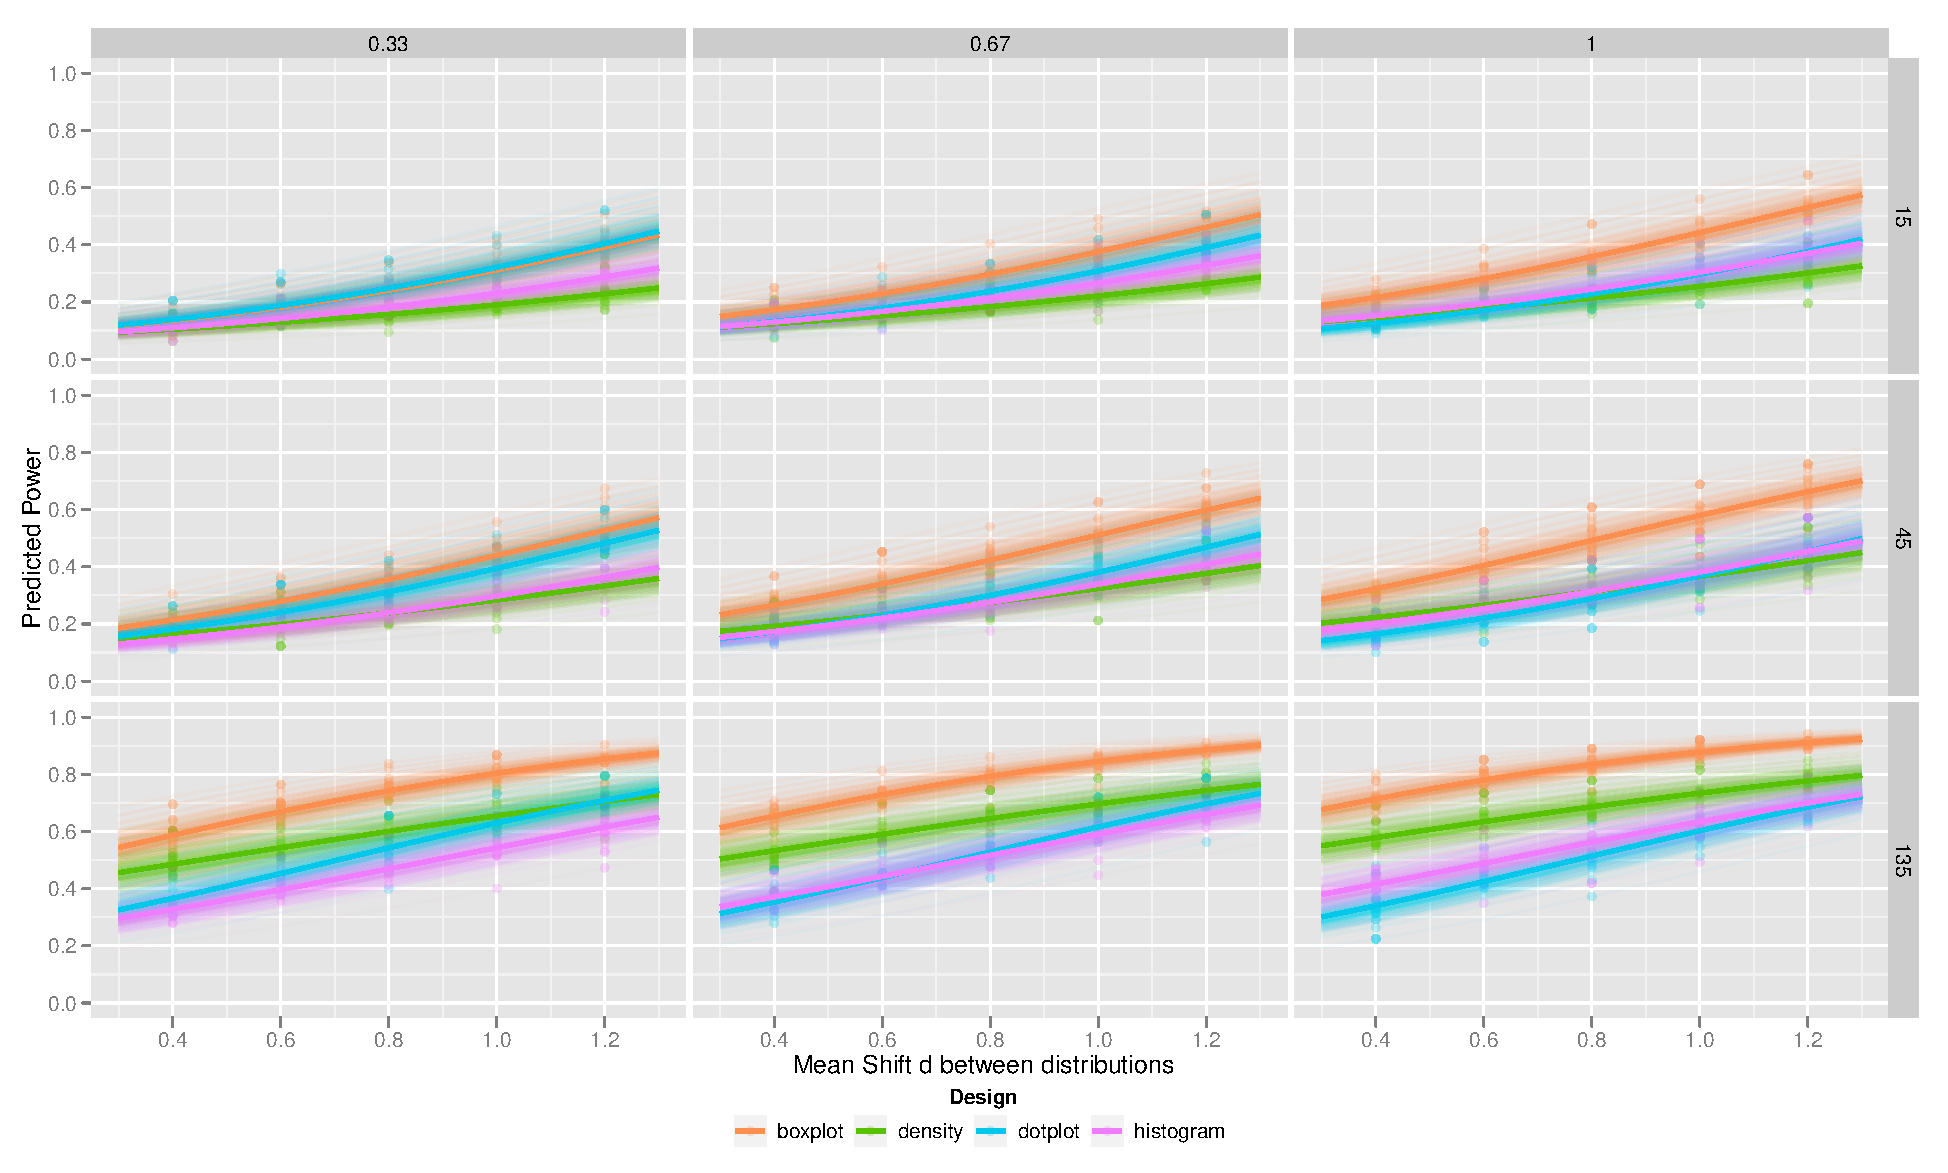
\includegraphics[width=0.9\linewidth]{power-exp2} 
\vspace{-0.2in}
   \caption{Overview of power predictions for the four different designs. The fully saturated thick lines show average predicted power for each of the designs facetted by size of the red group (top to bottom) and relative size of the blue group to the red group (left to right). Thin lines represent variability due to subject-specific abilities. }
   \label{fig:power2}
\end{figure*}

Time taken to answer was log transformed before the modeling process to de-emphasize the impact of very large values (up to 500 seconds). The findings are consistent with correctness - time taken shows big differences between polar and cartesian charts. 
The reference lines seem to increase the evaluation time, but not significantly. An increase in sample size decreases evaluation time, The inversion of the wave pattern at 180 degrees leads to a significant increase in time for cartesian charts, but not for polar charts (at least not significantly). Table \ref{tbl:time} shows an overview of the model parameters and estimates.

\begin{table}[ht]
\begin{center}
\resizebox{\linewidth}{!} {
%\rowcolors{2}{white}{lightgray}
\begin{tabular}{lrrrrrl}
  \hline
& & Estimate & Error & $t$-value & \multicolumn{2}{l}{approx $p$-value} \\   \hline
\bf design & intercept & 3.58 & 0.09 & 41.34 & 0.00 & ***\\ 
&  polar & 0.22 & 0.10 & 2.17 & 0.03 & * \\ [2pt]
\multicolumn{2}{l}{\bf covariates}\\
&reference line & 0.08 & 0.06 & 1.50 & 0.13 \\ [1pt]
 & sample size & -0.03 & 0.00 & -8.73 & 0.00 & ***\\ [1pt]
&  offset: 90 & -0.06 & 0.08 & -0.72 & 0.47 \\ 
& 180 & 0.16 & 0.08 & 2.07 & 0.04 & *\\ 
&  270 & -0.04 & 0.07 & -0.54 & 0.59 \\ [2pt]
\multicolumn{2}{l}{\bf interactions}\\
&  polar:line & -0.03 & 0.08 & -0.40 & 0.69 \\ [1pt]
&    polar:sample size & 0.03 & 0.01 & 6.25 & 0.00 & ***\\ [1pt]
&    polar:offset 90 & 0.14 & 0.11 & 1.23 & 0.22 \\ 
&    polar:offset 180 & -0.17 & 0.11 & -1.55 & 0.12 \\ 
&    polar:offset 270 & 0.17 & 0.11 & 1.50 & 0.13 \\ 
   \hline
\\[-5pt]
   \multicolumn{5}{l}{Signif. codes:  0 `***' 0.001 `**' 0.01 `*' 0.05 `.' 0.1}
\end{tabular}}
\end{center}
\vspace{-0.2in}
\caption{\label{tbl:time} Model output for linear mixed effects model of (log) time taken, barchart design is baseline. }
\end{table}

 Confidence levels are measured on a five point scale --- they are subjective assessments by the participant `how certain are you'. We model confidence using the same model structure as before, i.e. using sample size and offset as covariates and including up to two-way interactions,
While there is a difference between the designs - participants reported higher confidence in dealing with the cartesian lineups -- this is only  a trend (i.e. not significant at 5\% but below 10\%). The only significant effect on reported confidence level is the use of reference lines in polar coordinates: participants report an increase in confidence (0.31 $\pm$ 0.13, $p$ value = 0.01) when using the reference line. This, however, does not translate to a significant increase in accuracy of results, as we have seen before.

 Cartesian coordinates resulted in a significantly more accurate identification of the real data set in significantly shorter time.






%


%Cartesian coordinates performed better when speaking of efficiency in terms of accuracy and speed. 76.92\% of the Cartesian charts shown resulted in the a correct identification of the real data while only 20.31\% of the polar charts did the same. A t-test comparing means for charts with polar coordinates versus charts with Cartesian coordinates resulted in a t statistic of 15.2013 with a p-value of 2.2e-16. Similarly, a t-test comparing means of time spent on charts with Cartesian coordinates versus charts with polar coordinates resulted in a p-value of 1.014e-11. The average of the log of time spent on each individual chart for charts with Cartesian coordinates is 3.53 minutes while it was 4.07 minutes for charts with polar coordinates. Cartesian coordinates resulted in a significantly more accurate identification of the real data set in significantly shorter time. 

%\begin{figure}[htbp] %  figure placement: here, top, bottom, or page
%   \centering
%   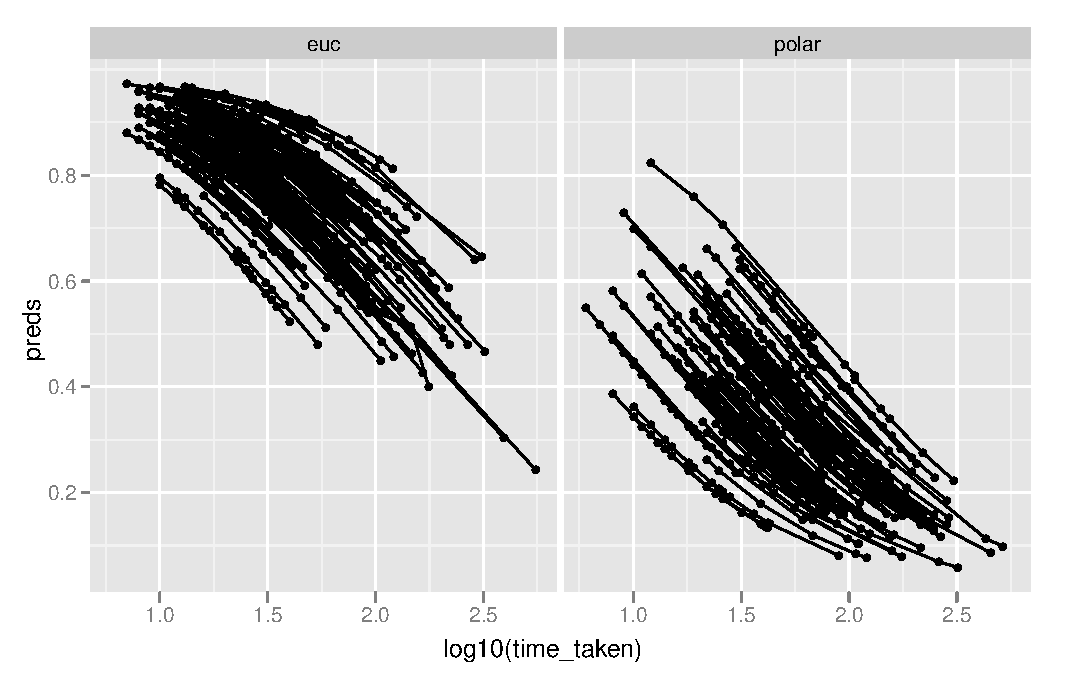
\includegraphics[width=3in]{turk4_time_perc_preds.pdf}  
%   \caption{Values predicted from XXXX how to say itXXXX of accuracy for log of time taken and test parameter.}
%   \label{accuracy_preds}
%\end{figure}
%
%Figure \ref{accuracy_preds} shows predicted accuracy levels. These predicted values were obtained by using R package lme4 and a mixed effect model explaining correct responses by type of chart and the log of time spent while accounting for different levels of accuracy for each individual who participated in the experiment. The predicted values show that there is an overall higher accuracy level for cartesian coordinates when compared to polar coordinates. For both chart types, as the time spent increases, the predicted accuracy decreases. 
%
%\begin{figure}[htbp] %  figure placement: here, top, bottom, or page
%   \centering
%   %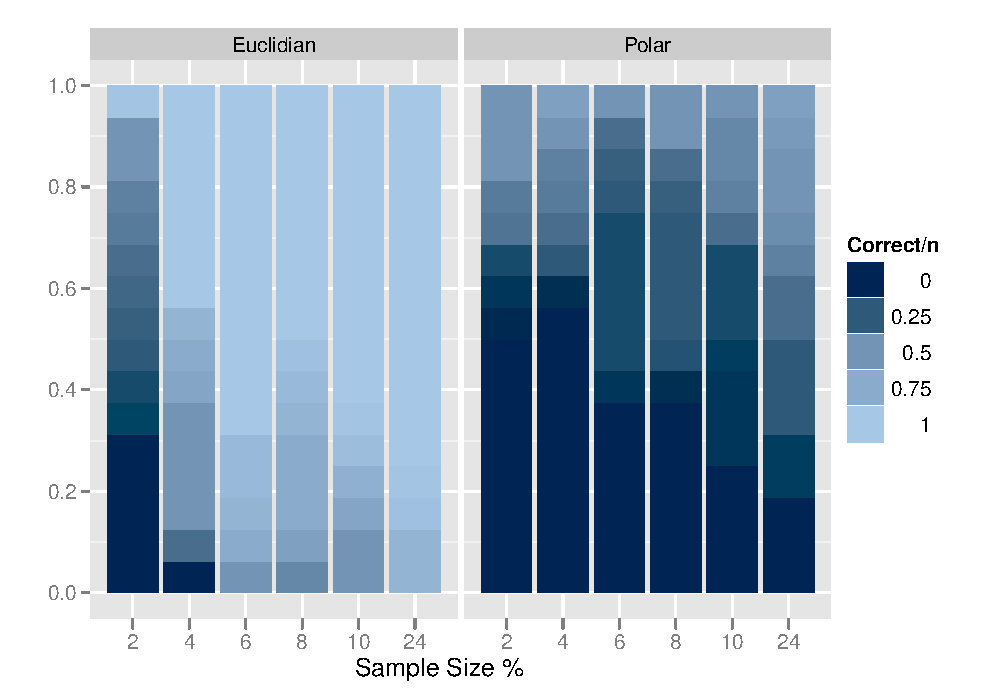
\includegraphics[width=3in]{turk4_samplesize_correctn.pdf}  
%   \caption{For each sample size for polar and cartesian coordinates, the bars are colored according to the number of correct responses. Darker colors indicate lower accuracy levels while lighter colors indicate higher accuracy levels. }
%   \label{samp_size_acc}
%\end{figure}

%Ideally, efficient detection of data characteristics will be possible at small sample sizes. The difficulty of the charts is largely determined by the sample size taken from the original data set. Samples of 24 \% generally result in higher accuracy as the extra information facilitates detection of a relationship. Figure \ref{accuracy_preds} shows the relationship between the number of correct responses relative to the total number of responses and how this relationship differs between cartesian and polar coordinates. The bars in the cartesian plot are overall a lighter color than they are in the polar plot. This indicates a higher level of accuracy at all sample sizes. For cartesian coordinates, we can see a stair step pattern in the accuracy levels as sample size increases. Lower levels of accuracy, indicated by darker colors, become consistently less prevalent as sample size increases. The relationship between sample size and accuracy level is not as simple for polar coordinates. Sample sizes of 2\% and 4\% have very similar accuracy levels. After 6\% the stair step pattern becomes visible and similar to that of cartesian coordinates. Sample size seems to have less of an effect on accuracy for polar coordinates than it does for cartesian coordinates. Predicted values of the proportion of correct responses when explained by sample size, the type of chart, and the interaction between these two factors, show that there is a significant difference between the relationship between sample size and correct responses for polar and cartesian coordinates. Indeed, the proportion of correct responses increases more rapidly as sample size increases for cartesian coordinates than it does for polar coordinates. 
%
%The effect of a reference line on accuracy and time was not statistically significant for both types of charts. When looking at plots of the data, however, the time spent on the charts seems to be higher when there is a reference line.This is true for both cartesian and polar charts. Also visible in the data is a slight increase in accuracy with the presence of a reference line. These characteristics can be seen in figure\ref{reflines}.  
%
%\begin{figure}[htbp] %  figure placement: here, top, bottom, or page
%   \centering
%   %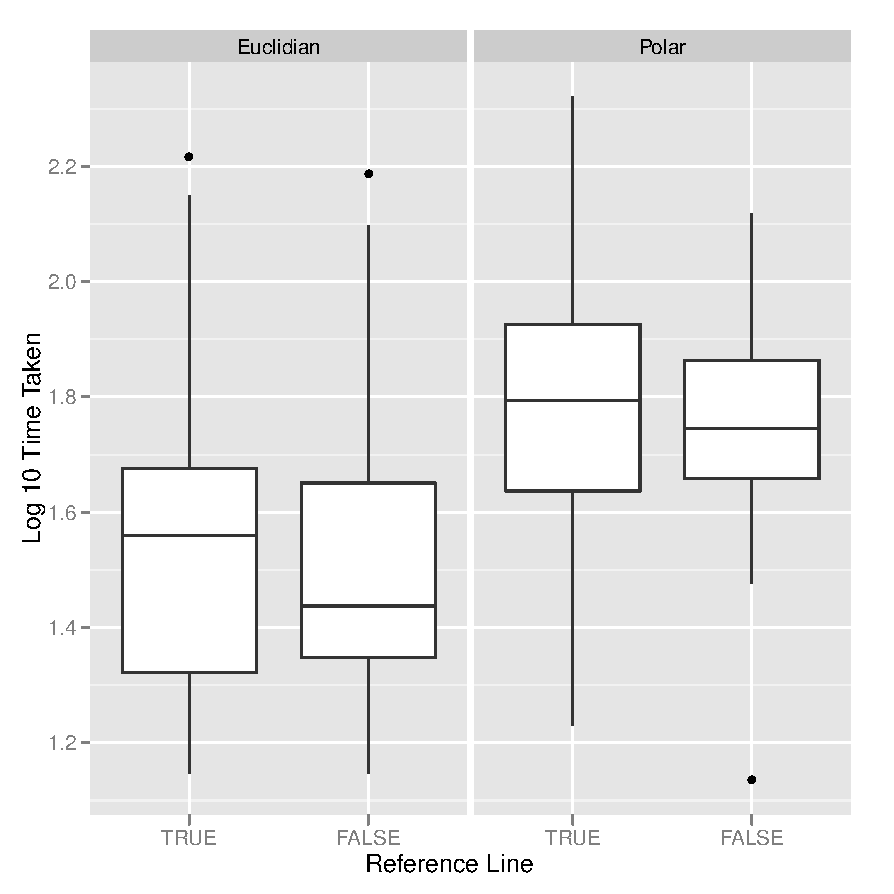
\includegraphics[width=1.5in]{turk4_refilne_time.pdf}  
%   %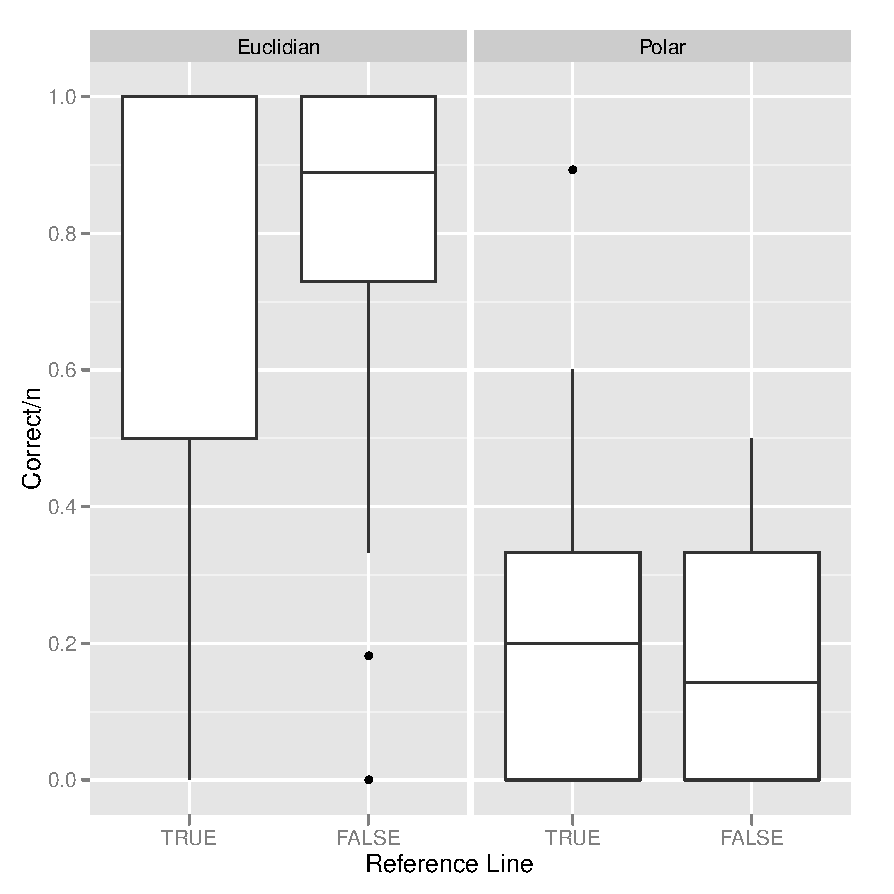
\includegraphics[width=1.5in]{turk4_refline_correctn.pdf}  
%   \caption{The relationship between reference line and time spent (left) and the relationship between reference line and accuracy (right). Although not statistically significant, some patterns are visible.}
%   \label{reflines}
%\end{figure}



